% 建议使用 XeLaTeX 或 LuaLaTeX 编译(中文与公式支持更佳)
\documentclass[UTF8,zihao=-4]{ctexart}

\usepackage[a4paper,margin=2.5cm]{geometry}
\usepackage{amsmath, amssymb, amsthm}
\usepackage{bm}
\usepackage{hyperref}
\usepackage{graphicx}
\usepackage{caption}
\usepackage{listings}
\usepackage{xcolor}
\usepackage{float}
\usepackage{placeins}
\graphicspath{{figures/}}

\lstdefinestyle{code}{
  basicstyle=\ttfamily\small,
  numbers=left,
  numberstyle=\tiny,
  numbersep=8pt,
  keywordstyle=\color{blue},
  commentstyle=\color{teal!70!black},
  stringstyle=\color{orange!70!black},
  showstringspaces=false,
  breaklines=true,
  frame=single,
  framerule=0.3pt,
  rulecolor=\color{black!15}
}
\lstset{style=code}

\title{深度确定性策略梯度(DDPG):原理、公式、应用与实战}
\author{}
\date{\today}

\begin{document}
\maketitle

\section{引言}
深度确定性策略梯度(Deep Deterministic Policy Gradient,DDPG)将确定性策略梯度与深度神经网络结合,通过经验回放与目标网络稳定训练过程,适用于连续动作控制任务。算法同时学习确定性策略(Actor)与动作价值函数(Critic),实现高效的离策略学习。

\section{原理与公式}
\subsection{确定性策略梯度}
对于确定性策略 \(\mu_\theta(s)\) 与评论家 \(Q_w(s,a)\),梯度形式为:
\begin{equation}
\nabla_\theta J(\theta) = \mathbb{E}_{s \sim \mathcal{D}}\big[ \nabla_a Q_w(s,a)|_{a=\mu_\theta(s)} \nabla_\theta \mu_\theta(s) \big],
\end{equation}
其中样本来自回放缓存 \(\mathcal{D}\),允许离策略更新。

\subsection{评论家更新}
评论家利用目标网络 \((\mu_{\theta^-}, Q_{w^-})\) 计算 TD 目标:
\begin{equation}
L(w) = \mathbb{E}\Big[\big(r + \gamma Q_{w^-}(s', \mu_{\theta^-}(s')) - Q_w(s,a)\big)^2\Big].
\end{equation}
目标网络采用软更新 \(\theta^- \leftarrow \tau \theta + (1-\tau)\theta^-\),缓解估计震荡。

\subsection{探索噪声}
由于策略确定性,需额外噪声促进探索:\(a_t = \mu_\theta(s_t) + \mathcal{N}_t\)。常用 OU 噪声或高斯噪声保持动作的时间连续性。

\section{应用与技巧}
\begin{itemize}
  \item \textbf{机器人控制}:连续扭矩或轨迹规划。
  \item \textbf{工业控制}:调节连续阀门、温度、压力等执行量。
  \item \textbf{自动驾驶仿真}:联合学习转向、油门等连续指令。
  \item \textbf{实用建议}:使用大容量回放缓存,规范化观测,裁剪梯度,调节噪声尺度,持续监控评论家损失避免崩塌。
\end{itemize}

\section{Python 实战}
脚本 \texttt{gen\_ddpg\_figures.py} 在一维连续控制任务上训练简化的 DDPG,展示回报曲线与策略函数随状态的变化。
\begin{lstlisting}[language=Python,caption={脚本 gen_ddpg_figures.py 片段}]
q_pred = critic_w @ features(state, action)
q_target = reward + gamma * critic_target_w @ features(next_state, actor_target(next_state))
critic_w += critic_lr * (q_target - q_pred) * features(state, action)

grad_q = critic_grad(state, actor(state))
actor_theta += actor_lr * grad_q
\end{lstlisting}

\section{实验结果}
\begin{figure}[H]
  \centering
  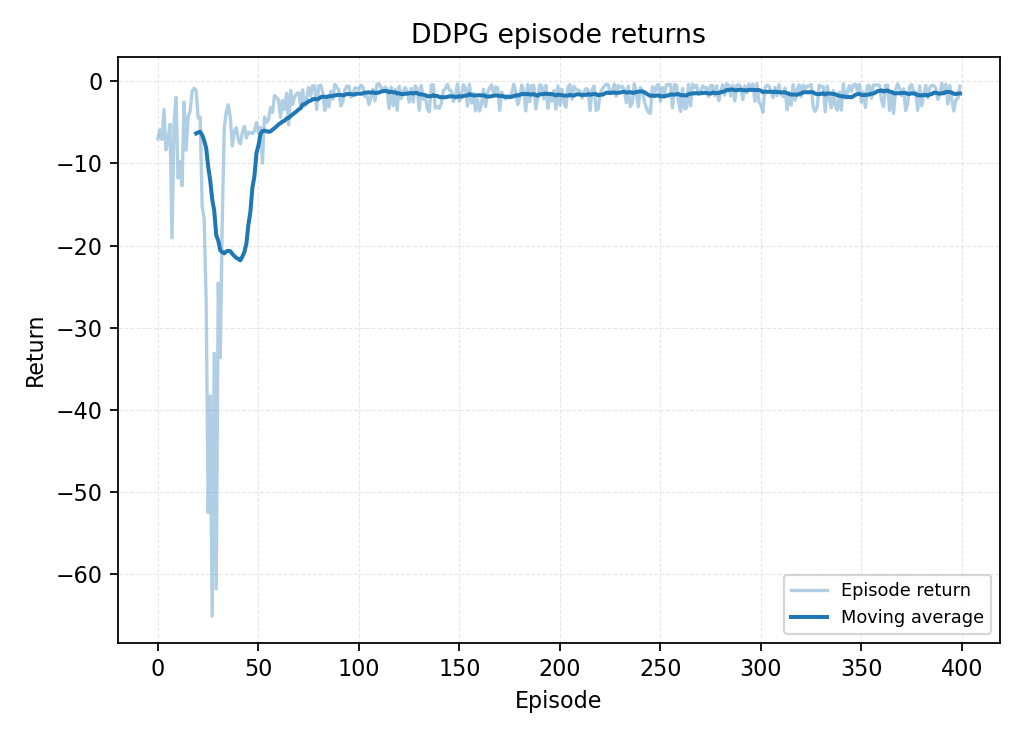
\includegraphics[width=0.8\linewidth]{ddpg_returns.png}
  \caption{DDPG 训练过程中的回报提升}
  \label{fig:ddpg_returns_cn}
\end{figure}

\begin{figure}[H]
  \centering
  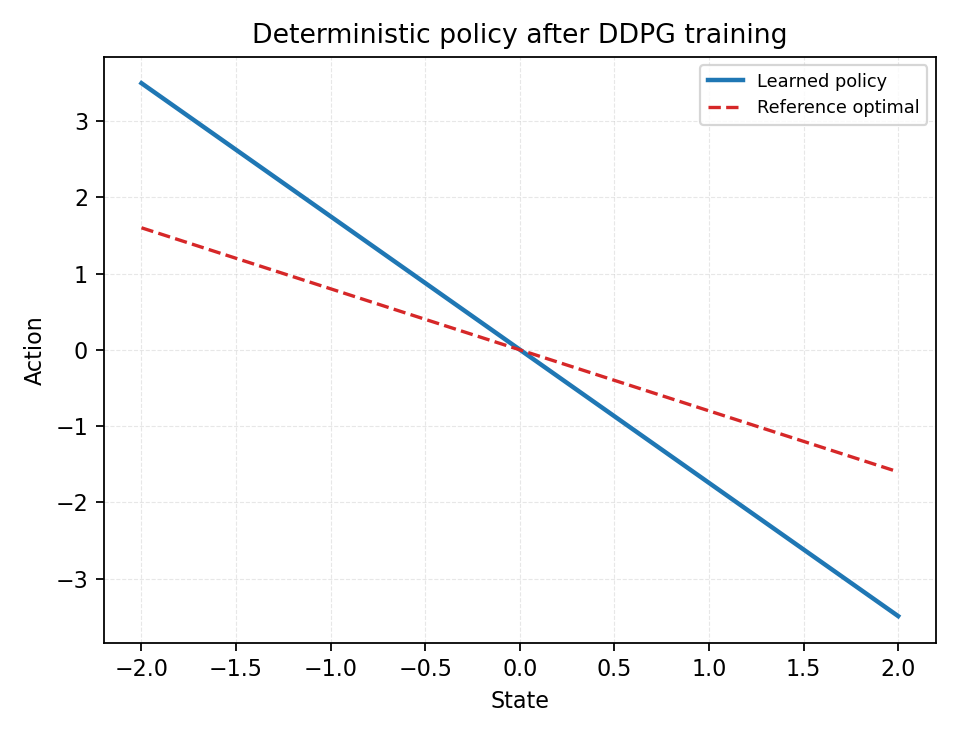
\includegraphics[width=0.82\linewidth]{ddpg_policy_trace.png}
  \caption{训练后策略在不同状态下的动作输出,与最优动作对比}
  \label{fig:ddpg_policy_trace_cn}
\end{figure}

\FloatBarrier
\section{总结}
DDPG 通过目标网络与回放缓冲稳定确定性策略梯度学习。恰当的探索噪声、数据规范化和评论家监控是成功应用的关键。示例展示了回报的提升以及策略逐渐逼近最优连续动作。

\end{document}